\documentclass[12pt]{article}
\usepackage[a4paper,margin=1.25cm]{geometry}
\usepackage{amsmath,amssymb,mathtools}
\usepackage{graphicx}
\usepackage{booktabs}
\usepackage{tabularx}
\usepackage{tikz}
\usepackage[T1]{fontenc}
\usepackage[utf8]{inputenc}
\usepackage[english]{babel}

\setlength{\parindent}{0pt}
\setlength{\parskip}{0.45em}
\setlength{\abovedisplayskip}{5pt plus 1pt minus 1pt}
\setlength{\belowdisplayskip}{5pt plus 1pt minus 1pt}
\setlength{\abovedisplayshortskip}{3pt plus 1pt minus 1pt}
\setlength{\belowdisplayshortskip}{3pt plus 1pt minus 1pt}

\newcommand{\dd}{\,\mathrm{d}}
\newcommand{\ii}{\mathrm{i}}
\newcommand{\e}{\mathrm{e}}
\newcommand{\Arg}{\operatorname{Arg}}
\newcommand{\Ip}{\operatorname{Im}}
\newcommand{\lc}{\ell}

\begin{document}

\begin{center}
{\Large\bfseries Two symmetries of the circle and an elliptic angle}\\[0.35em]
{\large a line integral evaluated without ever computing it}
\end{center}

\textbf{Problem.} Let \(D=\{x^2+y^2<1\}\) and let \(\lc=\partial D\) be
traversed once counterclockwise. Prove
\[
\oint_{\lc}\frac{x\e^{\sin y}\dd y-y\e^{-\sin x}\dd x}{4x^2+5y^2}
=\oint_{\lc}\frac{x\e^{-\sin y}\dd y-y\e^{\sin x}\dd x}{5x^2+4y^2},
\tag{I}
\]
\[
\oint_{\lc}\frac{x\e^{\sin y}\dd y-y\e^{-\sin x}\dd x}{4x^2+5y^2}
>\frac{53\pi}{120}.
\tag{II}
\]

\[
\boxed{\displaystyle
\text{(I) by the reflection }(x,y)\mapsto(y,x);
\qquad
\text{(II) by the antipode }(x,y)\mapsto(-x,-y)
\text{ and }
\oint_{\lc}\frac{x\dd y-y\dd x}{4x^2+5y^2}=\frac{\pi}{\sqrt5}.}
\]

\textbf{Overview.}
Neither integral can be evaluated in closed form, and neither needs to
be. Two isometries of the circle do everything.

The reflection \(S(x,y)=(y,x)\) maps \(\lc\) to itself with reversed
orientation and carries the second differential form to minus the first;
the two sign changes cancel, which is (I).

The antipodal map \(A(x,y)=(-x,-y)\) preserves \(\lc\) \emph{with} its
orientation and replaces \(\e^{u}\) by \(\e^{-u}\). Averaging the form
with its pullback therefore turns both exponentials into \(\cosh\), and
\(\cosh\ge1\) gives a clean lower bound by the ``elliptic angle form''
\(\frac{x\dd y-y\dd x}{4x^2+5y^2}\). That form is
\(\frac1{2\sqrt5}\dd\Arg(2x+\ii\sqrt5y)\), and the image of the unit
circle under \((x,y)\mapsto(2x,\sqrt5y)\) winds once around the origin,
so the integral is \(\frac{2\pi}{2\sqrt5}=\frac{\pi}{\sqrt5}\). Finally
\(\frac1{\sqrt5}>\frac{53}{120}\).

Write
\[
\omega=\frac{x\e^{\sin y}\dd y-y\e^{-\sin x}\dd x}{4x^2+5y^2},
\qquad
\eta=\frac{x\e^{-\sin y}\dd y-y\e^{\sin x}\dd x}{5x^2+4y^2},
\]
and \(I=\oint_\lc\omega\), \(J=\oint_\lc\eta\).

\section*{1. The integrals in parametric form}

With the standard positive parametrisation
\[
x=\cos t,\quad y=\sin t,\quad
\dd x=-\sin t\dd t,\quad \dd y=\cos t\dd t,
\qquad 0\le t\le2\pi,
\]
abbreviate \(c=\cos t\), \(s=\sin t\). Then
\[
x\e^{\sin y}\dd y=c^2\e^{\sin s}\dd t,
\qquad
-y\e^{-\sin x}\dd x=s^2\e^{-\sin c}\dd t,
\]
so
\[
I=\int_0^{2\pi}\frac{c^2\e^{\sin s}+s^2\e^{-\sin c}}{4c^2+5s^2}\dd t,
\qquad
J=\int_0^{2\pi}\frac{c^2\e^{-\sin s}+s^2\e^{\sin c}}{5c^2+4s^2}\dd t .
\tag{1}
\]
Both integrands are continuous and positive, so \(I,J>0\); the
denominators vanish only at the origin, which is not on \(\lc\).

\section*{2. Part (I): the reflection \(x\leftrightarrow y\)}

Let \(S(x,y)=(y,x)\), the reflection in the diagonal. It maps the unit
circle onto itself but reverses orientation:
\[
S(\lc)=-\lc .
\tag{2}
\]
Its pullback substitutes \(x\mapsto y\), \(y\mapsto x\),
\(\dd x\mapsto\dd y\), \(\dd y\mapsto\dd x\) in \(\eta\):
\[
S^{*}\eta
=\frac{y\e^{-\sin x}\dd x-x\e^{\sin y}\dd y}{5y^2+4x^2}
=-\frac{x\e^{\sin y}\dd y-y\e^{-\sin x}\dd x}{4x^2+5y^2}
=-\omega .
\tag{3}
\]
The change-of-variables rule for line integrals gives
\(\int_{S(\lc)}\eta=\int_{\lc}S^{*}\eta\), so by (2) and (3)
\[
-\oint_{\lc}\eta=-\oint_{\lc}\omega
\qquad\Longrightarrow\qquad
\boxed{I=J.}
\]

The same statement without the language of forms: in (1) substitute
\(t\mapsto\frac\pi2-t\), which exchanges \(\cos\) and \(\sin\). The
denominator \(5c^2+4s^2\) becomes \(4c^2+5s^2\), the numerator of \(J\)
becomes the numerator of \(I\), and the two integrals over the full
period coincide.

\section*{3. Why Green's theorem is the wrong first move}

The natural reflex is to apply Green's theorem to \(\omega\) over \(D\).
It does not apply: the denominator \(4x^2+5y^2\) vanishes at the origin,
which lies inside \(D\), so the field is not \(C^1\) on the region.

One can excise a small disk around the origin, apply Green's theorem to
the annulus, and let the radius tend to zero. But then the boundary
term at the small circle must be evaluated, and it is exactly the
quantity one is after. The symmetries below are cleaner because they
never leave the circle.

\section*{4. Part (II): the antipodal map produces \(\cosh\)}

Let \(A(x,y)=(-x,-y)\), the rotation by \(\pi\). It preserves the unit
circle \emph{and} its orientation:
\[
A(\lc)=\lc .
\]
Since \(\sin\) is odd and the denominator is even,
\[
A^{*}\omega=\frac{x\e^{-\sin y}\dd y-y\e^{\sin x}\dd x}{4x^2+5y^2},
\tag{4}
\]
and \(\oint_\lc\omega=\oint_\lc A^{*}\omega\). Averaging,
\[
I=\frac12\oint_{\lc}\bigl(\omega+A^{*}\omega\bigr),
\qquad
\frac{\omega+A^{*}\omega}{2}
=\frac{x\cosh(\sin y)\dd y-y\cosh(\sin x)\dd x}{4x^2+5y^2},
\tag{5}
\]
using \(\frac{\e^{u}+\e^{-u}}{2}=\cosh u\).

On the unit circle both differentials appearing in (5) are
\emph{non-negative}:
\[
x\dd y=c^2\dd t\ge0,
\qquad
-y\dd x=s^2\dd t\ge0 .
\]
Therefore \(\cosh\ge1\) may be applied termwise:
\[
I=\int_0^{2\pi}\frac{c^2\cosh(\sin s)+s^2\cosh(\sin c)}{4c^2+5s^2}\dd t
\ \ge\
\int_0^{2\pi}\frac{c^2+s^2}{4c^2+5s^2}\dd t
=\oint_{\lc}\frac{x\dd y-y\dd x}{4x^2+5y^2}.
\tag{6}
\]

\textbf{This is not a pointwise bound on the original integrand.} At
individual points the integrand of \(I\) is smaller than the base
integrand, because \(\e^{-\sin c}<1\) wherever \(\sin c>0\). The
inequality appears only after averaging the values at the antipodal pair
\(t\) and \(t+\pi\), where the two exponentials are reciprocals and their
mean is a \(\cosh\).

\section*{5. The base integral is an angle}

Let
\[
K=\oint_{\lc}\frac{x\dd y-y\dd x}{4x^2+5y^2}.
\]
Apply the linear stretch
\[
u=2x,\qquad v=\sqrt5\,y,\qquad W=u+\ii v=2x+\ii\sqrt5\,y,
\]
so that \(u^2+v^2=4x^2+5y^2\). For any \(W\ne0\),
\[
\dd\Arg W=\Ip\frac{\dd W}{W}=\frac{u\dd v-v\dd u}{u^2+v^2},
\]
and here \(\dd u=2\dd x\), \(\dd v=\sqrt5\dd y\), so
\[
u\dd v-v\dd u=2\sqrt5\bigl(x\dd y-y\dd x\bigr).
\]
Hence
\[
\boxed{\displaystyle
\frac{x\dd y-y\dd x}{4x^2+5y^2}
=\frac1{2\sqrt5}\dd\Arg\bigl(2x+\ii\sqrt5\,y\bigr).}
\tag{7}
\]
As \((x,y)\) traverses the unit circle once, the point
\[
W(t)=2\cos t+\ii\sqrt5\sin t
\]
traverses an ellipse once around the origin, so its argument increases by
\(2\pi\) and
\[
K=\frac{1}{2\sqrt5}\cdot2\pi=\frac{\pi}{\sqrt5}.
\tag{8}
\]

\begin{center}
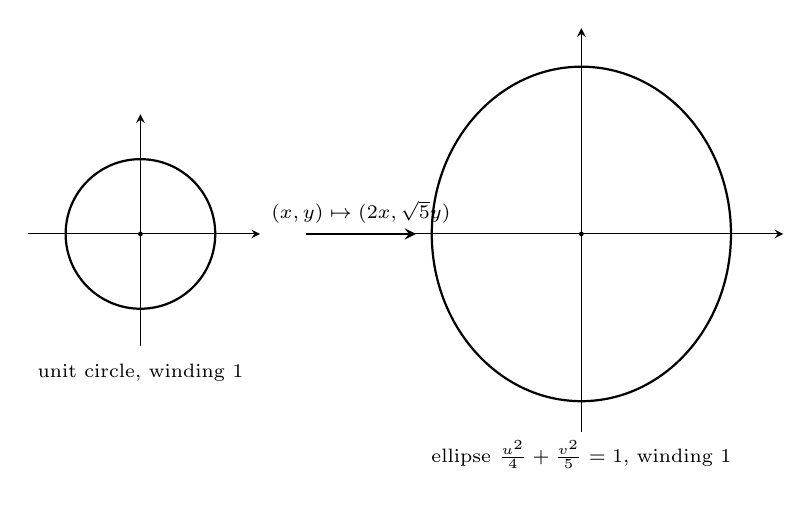
\begin{tikzpicture}[>=stealth]
\begin{scope}[scale=0.95]
  \draw[->] (-1.5,0)--(1.6,0); \draw[->] (0,-1.5)--(0,1.6);
  \draw[thick] (0,0) circle (1);
  \fill (0,0) circle (0.9pt);
  \node at (0,-1.85) {\scriptsize unit circle, winding \(1\)};
\end{scope}
\draw[->,thick] (2.1,0)--(3.5,0)
  node[midway,above] {\scriptsize \((x,y)\mapsto(2x,\sqrt5y)\)};
\begin{scope}[shift={(5.6,0)},scale=0.95]
  \draw[->] (-2.6,0)--(2.7,0); \draw[->] (0,-2.65)--(0,2.75);
  \draw[thick] (0,0) ellipse (2 and 2.2360679);
  \fill (0,0) circle (0.9pt);
  \node at (0,-2.95) {\scriptsize ellipse \(\frac{u^2}{4}+\frac{v^2}{5}=1\), winding \(1\)};
\end{scope}
\end{tikzpicture}
\end{center}

Geometrically, \(\frac{x\dd y-y\dd x}{x^2+y^2}\) measures the increment of
the ordinary polar angle. Replacing the denominator by \(4x^2+5y^2\)
measures instead the angle \emph{after} the stretch. The stretch turns
the circle into an ellipse, but the ellipse still encircles the origin
exactly once, since winding number is a topological invariant, so the
total increment is again \(2\pi\), only rescaled by
\(\frac1{2\sqrt5}\).

A direct check confirms (8): with \(c^2+s^2=1\),
\[
K=\int_0^{2\pi}\frac{\dd t}{4\cos^2t+5\sin^2t}
=\frac{2\pi}{2\cdot\sqrt5}=\frac{\pi}{\sqrt5},
\]
by the standard formula
\(\int_0^{2\pi}\frac{\dd t}{a^2\cos^2t+b^2\sin^2t}=\frac{2\pi}{ab}\)
with \(a=2\), \(b=\sqrt5\), itself just (7) in disguise.

\section*{6. Conclusion of part (II)}

From (6) and (8),
\[
I\ \ge\ \frac{\pi}{\sqrt5}.
\]
It remains to compare with \(\frac{53\pi}{120}\). Since all quantities
are positive,
\[
\frac1{\sqrt5}>\frac{53}{120}
\iff
120^2>5\cdot53^2
\iff
14400>14045,
\]
which is true. Hence
\[
\boxed{\displaystyle
I\ \ge\ \frac{\pi}{\sqrt5}=1.4049629\ldots
\ >\ \frac{53\pi}{120}=1.3875368\ldots,}
\]
which is (II).

The true value, by numerical quadrature of (1), is
\[
I=J=1.5580643\ldots,
\]
so the chain of bounds is comfortable: the \(\cosh\ge1\) step costs about
\(10\%\), and the rational comparison a further \(1.3\%\).

\begin{center}
\small
\renewcommand{\arraystretch}{1.35}
\begin{tabularx}{0.86\textwidth}{@{}Xll@{}}
\toprule
Quantity & Exact & Value \\
\midrule
The integral \(I=J\) & -- & \(1.5580643\) \\
After \(\cosh\ge1\) & \(\pi/\sqrt5\) & \(1.4049629\) \\
Target & \(53\pi/120\) & \(1.3875368\) \\
\bottomrule
\end{tabularx}
\end{center}

\section*{7. The elliptic angle as a Blaschke product}

This section is not needed for the proof; it identifies the complex
object behind the stretch.

On \(|z|=1\), with \(z=x+\ii y\), one has \(\bar z=z^{-1}\) and
\[
x=\frac{z+z^{-1}}{2},\qquad y=\frac{z-z^{-1}}{2\ii},
\]
so
\[
W=2x+\ii\sqrt5\,y=\frac{2+\sqrt5}{2}\,z+\frac{2-\sqrt5}{2}\,z^{-1}
=\frac{2+\sqrt5}{2}\,z^{-1}\bigl(z^2-\rho\bigr),
\tag{9}
\]
where
\[
\rho=-\frac{2-\sqrt5}{2+\sqrt5}=9-4\sqrt5=(\sqrt5-2)^2=0.0557\ldots<1 .
\]
Formula (9) makes the winding number transparent: on \(|z|=1\) the factor
\(z^{-1}\) contributes winding \(-1\), while \(z^2-\rho\) has its two
zeros \(z=\pm\sqrt\rho\) inside the disk and contributes \(+2\). The
total is \(+1\), confirming \(\Delta\Arg W=2\pi\) and hence (8).

Moreover \(\rho\in(0,1)\) means
\[
B(w)=\frac{w-\rho}{1-\rho w}
\]
is a Blaschke factor of the disk, and \(|z^2-\rho|=|1-\rho z^2|\) on
\(|z|=1\); the elliptic angle differs from the circular one by the
argument of a Blaschke product in \(z^2\). The eccentricity of the
ellipse and the modulus \(\rho\) of that Blaschke factor are two names
for the same number: \(\rho=\dfrac{b-a}{b+a}\) with \(a=2\),
\(b=\sqrt5\), since
\(\dfrac{\sqrt5-2}{\sqrt5+2}=(\sqrt5-2)^2=9-4\sqrt5\).

\section*{8. What generalises}

The proof used almost nothing about the specific functions.

\begin{center}
\small
\renewcommand{\arraystretch}{1.45}
\begin{tabularx}{\textwidth}{@{}>{\raggedright\arraybackslash}p{0.30\textwidth}X@{}}
\toprule
Ingredient & Property used \\
\midrule
\(\e^{\sin y}\), \(\e^{-\sin x}\)
& That the two exponents are odd and opposite, so that the antipodal
average is \(\cosh\ge1\). Any \(\e^{g(y)},\e^{-g(x)}\) with \(g\) odd
works. \\
\addlinespace
The denominators \(4x^2+5y^2\) and \(5x^2+4y^2\)
& That they are exchanged by \(x\leftrightarrow y\) (part I), and that
the first is a positive quadratic form (part II). \\
\addlinespace
The coefficients \(4,5\)
& Only through \(\sqrt{4\cdot5}=2\sqrt5\) in the final constant
\(\frac{\pi}{\sqrt5}=\frac{2\pi}{2\sqrt5}\). \\
\addlinespace
The unit circle
& That it is invariant under both \(S\) and \(A\), and that it winds once
around the origin. \\
\bottomrule
\end{tabularx}
\end{center}

Thus for any odd \(g\), any \(a,b>0\), and \(\lc\) the unit circle,
\[
\oint_{\lc}\frac{x\e^{g(y)}\dd y-y\e^{-g(x)}\dd x}{a^2x^2+b^2y^2}
\ \ge\ \frac{2\pi}{ab},
\]
with equality only for \(g\equiv0\). The stated problem is the case
\(g=\sin\), \(a=2\), \(b=\sqrt5\).

\end{document}
